\section{Quantum convolutional neural networks}
\label{sec:qcnn1}
As quantum CNNs have been studied and shown to have favourable properties (as discussed in \cref{sec:qcnn}), they are a reasonable choice to implement and test.
To do so, Qiskit's online tutorials \cite{qiskit_qcnn} were closely followed.

\subsection{Data}
To implement and test a quantum CNN, Qiskit's online tutorials were closely followed \cite{qiskit_qcnn}.
Being limited to few qubits, images with resolution $2\times4$ were generated, containing either vertical or horizontal with some Gaussian noise.
\Cref{fig:qcnn_data} shows examples thereof.
The task of the QCNN was to classify the images as either vertical or horizontal lines.

\begin{figure}
    \centering
    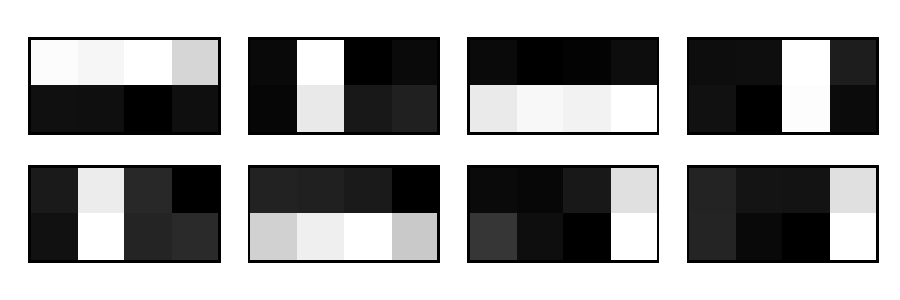
\includegraphics[width=\textwidth]{../code/qcnn/data.pdf}
    \caption{
        Data for the QCNN.
        With a total of 64 training images and 16 for testing, they form balanced dataset of $2\times4$ pixels, with either a vertical or horizontal line encoded as $1$ and $-1$.
        The images are generated with some Gaussian noise.
    }
    \label{fig:qcnn_data}
\end{figure}

\subsection{Model}
First, data is encoded using two repetitions of $Z$-angle encoding, implemented in Qiskit as the \texttt{ZFeatureMap}.
Each of the eight pixels of the image is mapped to a qubit through two repetitions of the Hadamard gate and $Z$-rotations parametrised by the pixel value being applied, in circuit notation:

\begin{equation}
    \begin{quantikz}
        \lstick{$\ket{0}$} & \gate{H} & \gate{R_Z(x_1)} & \gate{H} & \gate{R_Z(x_1)}  \\
        \lstick{$\ket{0}$} & \gate{H} & \gate{R_Z(x_2)} & \gate{H} & \gate{R_Z(x_2)}  \\
        \lstick{\vdots} \\
        \lstick{$\ket{0}$} & \gate{H} & \gate{R_Z(x_n)} & \gate{H} & \gate{R_Z(x_n)}  \\
    \end{quantikz}.
\end{equation}



The convolution layers act with pairwise parametrised rotations of neighbouring qubits, also wrapping around, entangling the first and last qubits through various CNOT gates and both parametrised and fixed $Z$- and $Y$-rotations.
Effectively, each consecutive pair of qubits were entangled by
\begin{equation}
    \begin{quantikz}
        &
        \qw
        &
        \targ{}
        &
        \gate{R_Z(\theta_{0})}
        &
        \ctrl{1}
        &
        \qw
        &
        \targ{}
        &
        \gate{R_Z(\pi/2)}
        &
        \qw
        \\
        &
        \gate{R_Z(-\pi/2)}
        &
        \ctrl{-1}
        &
        \gate{R_Y(\theta_{1})}
        &
        \targ{}
        &
        \gate{R_Y(\theta_{3})}
        &
        \ctrl{-1}
        &
        \qw
        &
        \qw
    \end{quantikz},
    \label{eq:qcnn_conv_gate}
\end{equation}
giving $3n$ parameters for each convolution layer of $n$ qubits.


Thereafter, pooling layers halve the active qubit counts by parametrised rotations and CNOT gates.
This is done by acting on the first and fifth, second and sixth et cetera with the following circuit:
\begin{equation}
    \begin{quantikz}
        &
        \qw
        &
        \targ{}
        &
        \gate{R_Z(\theta_{0})}
        &
        \ctrl{1}
        &
        \qw
        &
        \qw
        \\
        &
        \gate{R_Z(-\pi/2)}
        &
        \ctrl{-1}
        &
        \gate{R_Y(\theta_{1})}
        &
        \targ{}
        &
        \gate{R_Y(\theta_{3})}
        &
        \qw
    \end{quantikz},
\end{equation}
giving $3n/2$ parameters for each pooling layer of $n$ qubits.

For the final layer, the sole remaining qubit is measured, and the result is interpreted as the prediction.
In total, the circuit appears as in \cref{fig:qcnn_circuit} with a total of 63 parameters.

\begin{figure}
    \centering
    \begin{quantikz}[row sep={0.85cm,between origins}]
        \lstick[wires=8]{$\ket{0}^{\otimes 8}$}
        &
        \gate[wires=8, disable auto height]{{\rotatebox{90}{\texttt{ZFeatureMap}$(\bm{x})$}}}
        &
        \gate[wires=8, disable auto height]{{\rotatebox{90}{\text{Convolution}}}}
        &
        \gate[wires=8, disable auto height]{{\rotatebox{90}{\text{Pooling}}}}
        & \qw & \qw & \qw & \qw & \qw
        \\
        & \qw & \qw & \qw & \qw & \qw & \qw & \qw & \qw
        \\
        & \qw & \qw & \qw & \qw & \qw & \qw & \qw & \qw
        \\
        & \qw & \qw & \qw & \qw & \qw & \qw & \qw & \qw
        \\
        & & & &
        \gate[wires=4, disable auto height]{{\rotatebox{90}{\text{Convolution}}}}
        &
        \gate[wires=4, disable auto height]{{\rotatebox{90}{\text{Pooling}}}}
        & \qw & \qw & \qw
        \\
        & \qw & \qw & \qw & \qw & \qw & \qw & \qw & \qw
        \\
        & & & & & &
        \gate[wires=2, disable auto height]{{\rotatebox{90}{\text{Conv.}}}}
        &
        \gate[wires=2, disable auto height]{{\rotatebox{90}{\text{Pooling}}}}
        & \qw
        \\
        & & & & & & & & \meter{}
    \end{quantikz}
    \caption{
        Circuit diagram of the QCNN.
        Data is encoded using $Z$-angle encoding, before convolutional and pooling layers are applied.
        The final layer is a single qubit measurement.
    }
    \label{fig:qcnn_circuit}
\end{figure}


\subsection{Implementation}
As in Qiskit's guide, training was done using the COBYLA optimiser\footnote{Constrained Optimisation BY Linear Approximation.} which does not use gradients.
Why this optimiser was chosen is not clear, but testing shows that simulations using gradient based methods such as Adam or simple gradient descent is significantly slower.
However, as will be seen in \cref{sec:qcnn2}, that seems to have more to do with Qiskit's implementation than the optimiser itself.

\subsection{Results}
The accuracies and loss (mean square error) during training is shown in \cref{fig:qcnn_training}.
As in \cref{sec:qnn-vs-nn}, noise is modelled after the IBM Montreal hardware.
The networks were trained for 1000 epochs, and while neither reached full accuracy, the losses shrunk, indicating at least increased certainty in the predictions.
Interestingly, the noisy simulation appears to yield better predictions, despite suffering from higher losses during training.
It seems that the noiseless QCNN is overfitting to the training data, while the noisy QCNN generalises better.

\begin{figure}
    \centering
    \begin{subfigure}{0.49\textwidth}
        \centering
        \begin{tikzpicture}
            \begin{axis}[
                    width=\textwidth,
                    height=\textwidth,
                    xlabel={Iteration},
                    ylabel={MSE},
                    % legend pos=north west,
                    % legend style={at={(0.5,1.03)},anchor=north},
                    grid=major,
                    xtick distance=200,
                ]
                \addplot[mark=none, color=red] table[x=iteration, y=loss, col sep=comma] {../code/qcnn/noisy.csv};
                \addplot[mark=none, color=blue] table[x=iteration, y=loss, col sep=comma] {../code/qcnn/exact.csv};
                \legend{
                    Noisy QCNN,
                    Exact QCNN,
                }
            \end{axis}
        \end{tikzpicture}
        \caption{}
        \label{fig:qcnn_loss}
    \end{subfigure}
    \begin{subfigure}{0.49\textwidth}
        \centering
        \begin{tikzpicture}
            \begin{axis}[
                    width=\textwidth,
                    height=\textwidth,
                    xlabel={Iteration},
                    ylabel={Accuracy},
                    % legend pos=north west,
                    % legend style={at={(0.5,1.03)},anchor=north},
                    grid=major,
                    legend pos=south east,
                    xtick distance=200,
                ]
                % \addplot[mark=none, color=red] table[x=iteration, y=training_acc, col sep=comma] {../code/qcnn/noisy.csv};
                % \addplot[mark=none, color=red, dashed] table[x=iteration, y=test_acc, col sep=comma] {../code/qcnn/noisy.csv};
                % \addplot[mark=none, color=blue] table[x=iteration, y=training_acc, col sep=comma] {../code/qcnn/exact.csv};
                % \addplot[mark=none, color=blue, dashed] table[x=iteration, y=test_acc, col sep=comma] {../code/qcnn/exact.csv};
                \addplot[mark=none, color=red] table[x=iteration, y=train_mean_noisy, col sep=comma] {../code/qcnn/mean_accs.csv};
                \addplot[mark=none, color=red, dashed] table[x=iteration, y=test_mean_noisy, col sep=comma] {../code/qcnn/mean_accs.csv};
                \addplot[mark=none, color=blue] table[x=iteration, y=train_mean_exact, col sep=comma] {../code/qcnn/mean_accs.csv};
                \addplot[mark=none, color=blue, dashed] table[x=iteration, y=test_mean_exact, col sep=comma] {../code/qcnn/mean_accs.csv};
                \legend{
                    Noisy training,
                    Noisy test,
                    Exact training,
                    Exact test,
                }
            \end{axis}
        \end{tikzpicture}
        \caption{}
        \label{fig:qcnn_acc}
    \end{subfigure}
    \caption{
        Training of the basic QCNN.
        The red curves are for the noisy model (modelled after IBM's Montreal hardware), while the blue curves are for the exact model.
        The dashed curves are for the test set.
        (a) loss (mean square error) during training.
        (b) accuracy on the training and test sets (running mean with a 100 iteration window).
    }
    \label{fig:qcnn_training}
\end{figure}